\documentclass[a4paper, 11pt, titlepage]{article}
\usepackage{fancyhdr}
\usepackage{graphicx}
\usepackage{imakeidx}
\usepackage{makeidx}
\usepackage{mathtools}
\usepackage[spanish]{babel}
\usepackage{eurosym}
\usepackage{hyperref}
\usepackage{amssymb}
\usepackage{listings}
\usepackage{xcolor}
\usepackage{mathtools}
\usepackage{blkarray, bigstrut}
\usepackage{stackrel} 

\title{Tecnología de computadores}
\author{Francisco Javier Balón Aguilar}

\begin{document}

\maketitle
\renewcommand{\contentsname}{Índice}
\tableofcontents
\newpage

\section{Álgebra de Boole y puertas lógicas}

    El matemático y filósofo George Boole enunció una teoría matemática que permitía, de forma 
    algebráica, representar y operar con lógica preposicional. Una de sus características más 
    importantes es que las variables sólo podían tener dos valores: verdadero y falso. A esta 
    teoría se le conoce como Álgebra de Boole.

    Posteriormente, Claude E. Shannon, ingeniero electrónico, llega a la conclusión de que 
    es posible aplicar el Álgebra de Boole para el diseño, estudio y simplificación de circuitos 
    digitales. Uno de los factores que lo permiten son la simplificación a dos los valores de 
    las variables.

    El Álgebra de Boole queda definida, pues, por las siguientes reglas:

    \begin{itemize}
        \item Las variables sólo tienen dos posibles valores: 0 ó 1, es decir, utilizamos el 
        sistema de numeración binario.
        \item Operación de complementación o función NOT.
        \item Operación de suma lógica o función OR.
        \item Operación de producto lógico o función AND.
        \item Por convenio, el producto lógico es precedente a la suma lógica.
    \end{itemize}

    Estas operaciones algebráicas se implementan en los circuitos digitales mediante \textbf{puertas 
    lógicas}. Cada operación tiene asignada una puerta lógica.

    % TODO: poner gráfica con la representación de las puertas lógicas.

    Para representar los posibles resultados de la función lógica en función de las entradas se 
    utilizan las \textbf{tablas de verdad}. Ésta consta de una serie de columnas que representan 
    las variables de entrada y de salida, representando todas las combinaciones posibles de entradas.

    \begin{figure}[htp]
      \centering
      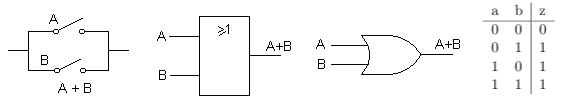
\includegraphics[width=1\textwidth]{resources/boole-or.png}
      \caption{Representación gráfica y tabla de verdad de la puerta lógica OR.}
      \label{boole-or}
    \end{figure}

    \begin{figure}[htp]
      \centering
      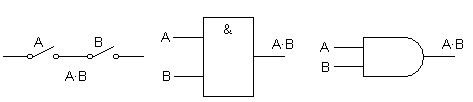
\includegraphics[width=1\textwidth]{resources/boole-and.png}
      \caption{Representación gráfica y tabla de verdad de la puerta lógica AND.}
      \label{boole-and}
    \end{figure}

    \begin{figure}[htp]
      \centering
      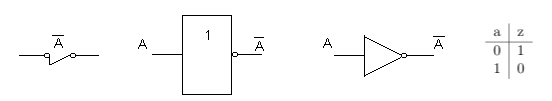
\includegraphics[width=1\textwidth]{resources/boole-not.png}
      \caption{Representación gráfica y tabla de verdad de la puerta lógica NOT.}
      \label{boole-not}
    \end{figure}

    Las puertas lógicas OR, AND y NOT son conocidas como funciones básicas (véanse figuras 
    \ref{boole-or}, \ref{boole-and} y \ref{boole-not}), cuyas operaciones cumplen las siguientes 
    propiedades:

    \begin{itemize}
      \item Conmutativa: $x+y=y+x$; $x\cdot y=y\cdot x$
      \item Elemento identidad: $x+0=x$; $x\cdot1=x$
      \item Propiedad distributiva: 
        \[x\cdot(y+x)=x\cdot y + x\cdot z\]
        \[x+(y\cdot z)=(x+y)\cdot(x+z)\]
      \item Elemento complementario: $x+\overline{x}=1$; $x\cdot\overline{x}=0$
      \item Propiedad de idempotencia: $x+x=x$; $x\cdot x=x$
      \item Elemento nulo: $x+1=1$; $x\cdot 0=0$
      \item Ley de convolución: $ \stackbin{=}{x}=x$
      \item Ley de absorción: $x+x\cdot y=x$; $x\cdot(x+y)=x$
      \item Propiedad asociativa: $x+(y+z)=(x+y)+z$; $x\cdot(y\cdot z)=(x\cdot y)\cdot z$
      \item Teorema del consenso:
        \[xy+\overline{x}z=xy+\overline{x}z+yz\]
        \[(x+y)(\overline{x}+z)=(x+y)(\overline{x}+z)(y+z)\] 
      \item Teorema de Morgan:
        \[\overline{x+y}=\overline{x}\cdot\overline{y}\]
        \[\overline{x\cdot y}=\overline{x}+\overline{y}\]
        \[x+\overline{x}y=x+y\]
        \[x\cdot(\overline{x}+y)=xy\]
    \end{itemize}

    Hay otras funciones que pueden realizarse como combinación de las funciones básicas, 
    siendo muy útiles en el diseño de circuitos digitales. Estas funciones son denominadas
    \textbf{funciones no básicas} (véanse figuras \ref{boole-nor}, \ref{boole-nand} y 
    \ref{boole-xor}).

    \begin{figure}[htp]
      \centering
      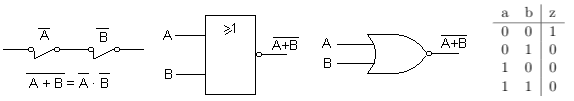
\includegraphics[width=1\textwidth]{resources/boole-nor.png}
      \caption{Representación gráfica y tabla de verdad de la puerta lógica NOR.}
      \label{boole-nor}
    \end{figure}

    \begin{figure}[htp]
      \centering
      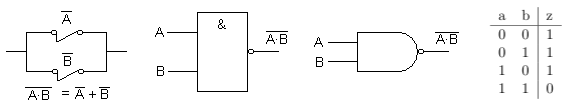
\includegraphics[width=1\textwidth]{resources/boole-nand.png}
      \caption{Representación gráfica y tabla de verdad de la puerta lógica NAND.}
      \label{boole-nand}
    \end{figure}

    \begin{figure}[htp]
      \centering
      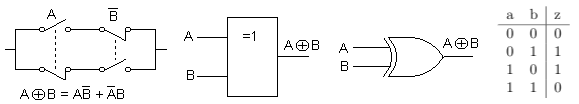
\includegraphics[width=1\textwidth]{resources/boole-xor.png}
      \caption{Representación gráfica y tabla de verdad de la puerta lógica XOR.}
      \label{boole-xor}
    \end{figure}

	\subsection{Forma canónica de las funciones lógicas}

		A partir de una función lógica podemos, mediante operaciones algebráicas, obtener 
		otras funciones lógicas equivalentes. O lo que es lo mismo, una función lógica puede 
		expresarse algebráicamente de muchas formas, siendo una de ellas la forma canónica.

		\subsubsection{Suma de minterms}

			La forma canónica de una función lógica expresada como suma de minterms\footnote{
				Un \textit{minterm} es un producto de todas las variables (negadas o sin negar)
				de una función lógica.

				Para saber si un \textit{minterm} va negado o no debemos observar si la entrada 
				es 0 ó 1; si es 0 la variable estará negado mientras que si es 1 la variable no 
				estará negada.
			} contiene la suma de todas las combinaciones de las entradas de tal forma que 
			la salida sea igual a 1.

		\subsubsection{Producto de maxterms}

			La forma canónica de una función lógica expresada como un producto de maxterms\footnote{
				Un \textit{maxterm} es una suma de todas las variables (negadas o sin negar) 
				de una función lógica.
			} contiene el producto de todas las combinaciones de las entradas que van a hacer que 
			la salida sea 0.

	\subsection{Simplificación de funciones lógicas}

		La simplificación consiste en la búsqueda de la función lógica que minimice el uso 
		de puertas lógicas. Una de las posibilidades consiste en utilizar los teoremas anteriormente 
		vistos.

		Ejemplo:
		\begin{gather*} 
			D = \overline{B}C + \overline{A}BC + ABC + \overline{A}B\overline{C} \\ 
			D = \overline{B}C + \overline{A}B\overline{C} + BC(\overline{A} + A) \\
			D = \overline{B}C + \overline{A}B\overline{C} + BC \\
			D = \overline{A}B\overline{C} + C(\overline{B} + B) \\
			D = \overline{A}B\overline{C} + C \\
			D = \overline{A}B+ C
		\end{gather*}

	\subsubsection{Homogeneización de puertas}

		Es posible implemnentar cualquier función lógica utilizando únicamente las puertas 
		NAND y NOR.

\end{document}